\chapter{Results and Discussion}\label{sec:resultsanddiscussion}

Some more general text
Why are some parts simulating and some parts using IBM?
All the code can be found on GitHub\textsuperscript[7]

\footnotetext[7]{Link to GitHub folder.}

\section{Simulating the qubit-based kNN algorithm}
\label{subsec:qubitKNNresults}

The computer used for the Liqui$\ket{}$ quantum simulations in this thesis only provides 8GB of RAM, thereby limiting the maximum number of simulated qubits to 24. Unfortunately, real-world machine learning problems usually involve large datasets that would require much more qubits such that a small artificial dataset needs to be constructed. For this reason, the classification of 9-bit, little-endian RGB colour codes into the classes \emph{red} and \emph{blue} will be considered. A 9-bit RGB colour code uses three bits to encode the content of each RGB colour; red, green and blue. Three binary bits $b_0,b_1,b_2$ can encode any of the numbers 0-7 according to the formula,

\begin{equation}
b_0*2^0 + b_1*2^1 + b_2*2^2 \text{ where } b_0,b_1,b_2 \in \left\{0,1\right\}
\end{equation}

For example, the 9-bit RGB code 111 100 100 can be written in roman numerals as 7,1,1 (full red, little green, little blue) and represents \colorbox{examplered}{this red tone}.

Since the class qubit $\ket{c}$ can only take binary values, class red is defined as $\ket{c} = \ket{0}$ and class blue is defined as $\ket{c} = \ket{1}$. The training set consists of 3 randomly chosen red and blue tones listed in Table~\ref{tab:trainingcolours}.

\begin{table}
\label{tab:trainingcolours}
\centering
    \begin{tabular}{| c| c |c |}
      %\toprule
      Colour & Binary 9-bit RGB string & Class\\
      \midrule
       \cellcolor{red1} & 111 000 000 & red ($\ket{0}$)\\\midrule
       \cellcolor{red2} & 101 000 000 & red ($\ket{0}$)\\\midrule
       \cellcolor{red3} & 110 000 000 & red ($\ket{0}$)\\\midrule
       \cellcolor{blue1} & 000 000 111 & blue ($\ket{1}$)\\\midrule
       \cellcolor{blue2} & 000 000 101 & blue ($\ket{1}$)\\\midrule
       \cellcolor{blue3} & 000 000 100 & blue ($\ket{1}$)\\\midrule
      \bottomrule
    \end{tabular}
    \caption{Training data set of six 9-bit RGB colour codes}
\end{table}

The quantum classifier will then be tested on four new colour tones (two red, two blue) listed in Table~\ref{tab:inputcolours}. Note that all training colours are either pure red colours (without green or blue content) or pure blue colours (without green or red content). The input colours, however, also include colours with additional green content testing how the classifier reacts in cases that are not included in the training set.

\begin{table}
\centering
    \begin{tabular}{| c| c |c |}
      %\toprule
      Colour & Binary 9-bit RGB string & Expected classification outcome\\
      \midrule
       \cellcolor{inputred1} & 100 000 000 & red ($\ket{0}$)\\\midrule
              \cellcolor{inputmixred2} & 110 100 000 & red ($\ket{0}$)\\\midrule

       \cellcolor{inputblue1} & 000 000 110 & blue ($\ket{1}$)\\\midrule
       \cellcolor{inputmixblue2} & 000 100 111 & blue ($\ket{1}$)\\\midrule
      \bottomrule
    \end{tabular}
    \label{tab:inputcolours}
    \caption{Input data set containing 9-bit RGB colour codes that require classification}
\end{table}

The first step towards the classification of RGB colour codes using the qubit-based kNN algorithm proposed by \citeA{Schuld2014} as described in detail in Section~\ref{subsubsec:quantumknearestneighbour} is preparing the initial superposition over all six 9-bit RGB training patterns $t^j$:

\begin{equation}
\label{equ:trainingsup}
\ket{T} = \frac{1}{\sqrt{6}}\sum_{j=1}^N \ket{t_1^j,t_2^j,...t_9^j;c^j}
\end{equation}

This can be done using the quantum state preparation algorithm by \citeA{Trugenberger2001} outlined in Section~\ref{subsubsec:classicaldataqubits}. In this case, the seven steps (see blue box in Section~\ref{subsubsec:classicaldataqubits}) of the state preparation algorithm have to be repeated six times in order to load the six RGB training patterns $t^j$ into the memory register $m$ defined in Equ.~\ref{equ:truginitial}. Afterwards, the state is given by,

\begin{equation}
\label{equ:trugcolours}
\ket{\phi_0} = \frac{1}{\sqrt{6}} \sum^6_{j=1} \ket{t^6_1,t^6_2,...,t^6_9;u_1=0,u_2=0;t^j_1,t^j_2,...,t^j_9}
\end{equation}

Equ.~\ref{equ:trugcolours} shows that the first register still contains the last stored RGB colour code $t^6$, the second register consists of the utility qubits $\ket{u_1}$ and $\ket{u_2}$ that are both in the \0 state and the last register is in an equal superposition over all six RGB training colours. Thus, besides the missing class qubit $\ket{c}$ the last register is in the desired superposition defined in Equ.~\ref{equ:trainingsup}.

In the next step of the quantum kNN the yet unclassified 9-bit RGB input pattern $x$ and an ancilla qubit $\ket{a}$ initialized in state \0 are added to the training superposition $\ket{T}$ to result in the full initial state $\ket{\psi_0}$:

\begin{equation}
\label{equ:fullinitialstate}
\ket{\psi_0} = \frac{1}{\sqrt{6}}\sum_{j=1}^6 \ket{x_1,x_2,...x_9;t_1^j,t_2^j,...t_9^j;c^j;0}
\end{equation}

The trick now is to realize that Equ.~\ref{equ:trugcolours} and ~\ref{equ:fullinitialstate} contain the same number of qubits. Firstly, each of them has nine qubits in the first register. Secondly, Equ.~\ref{equ:trugcolours} has two utility qubits that are balanced by the ancilla and the class qubit in Equ.~\ref{equ:fullinitialstate}. Lastly, there are again nine qubits in the third register in Equ.~\ref{equ:trugcolours} and the second register in Equ.~\ref{equ:fullinitialstate}. Thus, $\ket{\psi_0}$ and $\ket{\phi}$ both contain $9+9+2 = 20$ qubits. Since $\ket{\phi}$ is the current state of the qubits in the simulation, one simply needs to redefine the utility qubits such that the first one becomes the class qubit $\ket{u_1} = \ket{c^j}$ and the second utility qubit becomes the ancilla $\ket{u_2} = \ket{a}$. Note that class and ancilla qubit are currently still in the \0 state as indicated in the current quantum state $\ket{\phi_1}$:

\begin{equation}
\label{equ:trugcolours2}
\ket{\phi_1} = \frac{1}{\sqrt{6}} \sum^6_{j=1} \ket{t^6_1,t^6_2,...,t^6_9;c^j=0;a=0;t^j_1,t^j_2,...,t^j_9}
\end{equation}

Equ.~\ref{equ:trugcolours2} shows a quantum state with four registers as desired but the first register still contains the last training colour code $t^6$. However, it can simply be overwritten with the desired input pattern by comparing the two patterns and flipping qubits at positions where the patterns do not match up. For example, if the last training pattern was 000 000 100 and the input pattern is 000 000 110 one simply needs to flip the 8\textsuperscript{th} qubit through the application of an X gate. The state is now given by,

\begin{equation}
\label{equ:trugcolours3}
\ket{\phi_2} = \frac{1}{\sqrt{6}} \sum^6_{j=1} \ket{x_1,x_2,...,x_9;c^j=0;a=0;t^j_1,t^j_2,...,t^j_9}
\end{equation}

Currently, every training pattern is considered class $\ket{0}$ (red) which is of course incorrect. To flip the class qubit for the three training patterns encoding blue colours, one can make use of X and nCNOT gates. Consider the fourth (first blue) training pattern $t^4$ = 000 000 111 from Table~\ref{table:trainingcolours}. One might think that simply applying a 3CNOT($t_7,t_8,t_9$,c) gate controlled by the three qubits that are in the \1 state will suffice to flip the class label for this training pattern. However, depending on the classification problem at hand there might be another training pattern e.g. $t'$ = 111 110 111 belonging to class \0 for which the application of the 3CNOT($t_7,t_8,t_9$,c) gate would incorrectly flip the class qubit since the last three qubits of $t'$ are also in the \1 state.

To avoid this problem, apply an X gate to all qubits in the training pattern that are currently in the \0 state. Continuing the example with the training pattern $t^4$ = 000 000 111, X gates need to be applied to the first six qubits. The result is then $t^{4*}$ = 111 111 111. After this step, any other training pattern will contain at least one zero e.g. flipping the first six qubits of $t'$ = 111 110 111 results in $t'^{*}$ = 000 001 111. Hence, the training pattern $t^4$ is now the only pattern in the fourth register consisting only of ones. Now, this property can be exploited by applying a 9CNOT($t_1,t_2,...,t_9$,c) gate that will flip the class label to $\ket{1}$ for training pattern $t^4$ only. Acting X gates on the first six qubits again will restore all training patterns to their original states. Repeating this procedure for all training patterns belonging to class $\ket{1}$ (blue) entangles the class qubit $\ket{c}$ with the training patterns and the overall state is now described by,

\begin{equation}
\label{equ:trugcolours4}
\ket{\phi_3} = \frac{1}{\sqrt{6}} \sum^6_{j=1} \ket{x_1,x_2,...,x_9;c^j;a=0;t^j_1,t^j_2,...,t^j_9}
\end{equation}

Note that the class qubit is now not in the \0 state only. Inspection of Equ.~\ref{equ:trugcolours4} reveals that $\ket{\phi_3}$ is identical to the desired initial state $\ket{\psi_0}$ defined in Equ.~\ref{equ:fullinitialstate} the only difference being the position of the class and ancilla register. One can now proceed with the quantum kNN routine by simply putting the ancilla register into superposition with an H gate.

\begin{equation}
\label{equ:trugcolours5}
\ket{\phi_4} = \frac{1}{\sqrt{12}} \sum^6_{j=1} \Big[\ket{x_1,x_2,...,x_9;c^j;0;t^j_1,t^j_2,...,t^j_9} + \ket{x_1,x_2,...,x_9;c^j;1;t^j_1,t^j_2,...,t^j_9}\Big]
\end{equation}

The next step is the calculation of the HD between the input pattern and each training pattern which is done by the straightforward application of nine CNOT($x_s,t_s^j$) gates. By applying an X gate to every qubit in the fourth register the HD gets reversed as discussed in Section~\ref{subsubsec:quantumknearestneighbour}. The state is now,


\begin{align}
\ket{\phi_5} = \frac{1}{\sqrt{12}} \sum^6_{j=1} \prod_{s=1}^9 X(t^j_s)CNOT(x_s,t^j_s) \Big[&\ket{x_1,x_2,...,x_9;c^j;0;t^j_1,t^j_2,...,t^j_9}\notag\\
&+ \ket{x_1,x_2,...,x_9;c^j;1;t^j_1,t^j_2,...,t^j_9}\Big]
\end{align}
\begin{equation}
\quad\quad = \frac{1}{\sqrt{12}} \sum^6_{j=1} \Big[\ket{x_1,x_2,...,x_9;c^j;0;d_1^j,d_2^j,...d_9^j} + \ket{x_1,x_2,...,x_9;c^j;1;d_1^j,d_2^j,...d_9^j}\Big]
\end{equation}


In order to perform the sum over the fourth register and store the result in the complex phase of the corresponding term in the superposition one needs to implement the unitary operator $U$ previously defined in Equ.~\ref{equ:sumoperator} and \ref{equ:sumoperator2} with $n = 9$ in the case of 9-bit RGB classification. According to \citeA{Trugenberger2001} the operator $U$ can be decomposed as follows:

\begin{align}
&U\ket{\phi_5} = e^{-i\frac{\pi}{2n}K}\ket{\phi_5} = e^{-i\frac{\pi}{18}K}\ket{\phi_5} = \prod_{f=1}^{9} CL^{-2}(a,t_f) \prod_{k=1}^{9} L(t_k)\ket{\phi_5}\\
&\text{where } L = \begin{pmatrix}
e^{-i\frac{\pi}{18}} & 0 \\
0 & 1 
\end{pmatrix} \text{ and } CL^{-2} = \begin{pmatrix}
\mathbb{1} & 0 \\
0 & L^{-2}
\end{pmatrix}  \text{ and } L^{-2} = \begin{pmatrix}
e^{i\frac{\pi}{9}} & 0 \\
0 & 1
\end{pmatrix} \notag
\end{align}

The unitary gates $U$, $CU^{-2}$ and $U^{-2}$ can easily be defined in Liqui$\ket{}$'s programming environment and acting them on quantum state $\ket{\phi_5}$ leads to the result:

\begin{align}
\label{equ:trugcolours7}
\ket{\phi_6} = U\ket{\phi_5} = \frac{1}{\sqrt{12}} \sum^6_{j=1} \Big[&e^{i\frac{\pi}{18}d_H(\vec{x},\vec{v}^p)} \ket{x_1,x_2,...,x_9;c^j;0;d_1^j,d_2^j,...d_9^j} \notag\\
&+ e^{-i\frac{\pi}{18}d_H(\vec{x},\vec{v}^p)} \ket{x_1,x_2,...,x_9;c^j;1;d_1^j,d_2^j,...d_9^j}\Big]
\end{align}

In the last step, one simply has to act an H gate on the ancilla qubit in the third register which will transfer the total reverse HD from the phases into the amplitudes shown in Equ.~\ref{} below.

\begin{align}
\label{equ:trugcolours8}
\ket{\phi_7} = (\mathbb{1} \otimes \mathbb{1} \otimes H \otimes \mathbb{1})\ket{\phi_6} = \frac{1}{\sqrt{12}} \sum^6_{j=1} \Big[& cos\big[\frac{\pi}{18}d_H(\vec{x},\vec{t}^j)\big] \ket{x_1,x_2,...,x_9;c^j;0;d_1^j,d_2^j,...d_9^j} \notag\\
&+ sin\big[\frac{\pi}{18}d_H(\vec{x},\vec{t}^j)\big] \ket{x_1,x_2,...,x_9;c^j;1;d_1^j,d_2^j,...d_9^j}\Big]
\end{align}

At this point, the ancilla qubit in the third register is conditionally measured. This can be achieved with a simple if statement in F\# as shown in the pseudocode below:

\begin{Verbatim}[commandchars=\\\{\}]
if ancilla = 0 then
    measure class qubit
else
    start a new run
\end{Verbatim}

If and only if the ancilla is found to be in the \0 state, the class qubit is measured. The procedure is repeated for $y$ runs to gather sufficiently accurate statistics. Finally, the input vector is assigned to the most frequently measured class.

TO BE DONE!
Add table with the simulation results from Liqui$\ket{}$ and discuss them here.

It was shown that for this classification problem the quantum kNN algorithm by \citeA{Schuld2014} requires 20 qubits. Unfortunately, the IBM QC consists of only five qubits rendering an actual implementation of the 9-bit RGB colour classification impossible. Furthermore, even when the training and input patterns could be each encoded into two qubits, the algorithm would require 6 qubits making an IBM QC implementation again impossible. This can be seen from the initial state $\ket{\psi_0}$ in Equ.~\ref{equ:fullinitialstate} that contains the input pattern (two qubits), the training pattern (two qubits) as well as one class qubit and one ancilla qubit. This stresses the need for an alternative version of the quantum kNN algorithm based on amplitude-encoded data. 

\newpage

\section{Development of an amplitude-based kNN algorithm}
\label{subsec:amplitudeKNNalgorithm}

%(IBM doesn't allow for qubit based kNN due to restriction in qubit number need for a new algorithm based on amplitudes
%As an alternative to the qubit-based kNN algorithm
%quantum simulations of the qubit-based kNN algorithm 
%shortcomings )

To enable an implementation of the quantum kNN algorithm using the IBM Quantum Experience platform a new amplitude-based kNN algorithm was developed for this thesis. This algorithm by \citeA{SchuldFingerhuth} will be introduced in this section using colours for input \& training vectors and classes $A$ and $B$ based on the schematic Fig.~\ref{fig:knnconcept} in Section~\ref{subsubsec:knearestneighbour}.

\begin{bluebox}
The algorithm starts with the assumption that the following initial state can be constructed from $M$ training vectors with $N$ entries:

\begin{equation}
\label{equ:ampinitial}
\ket{\psi_0} = \frac{1}{\sqrt{2M}}\sum_{m=1}^{M} (\textcolor{emerald}{\ket{0}}\ket{\textcolor{red}{\Psi_{x}}}+\textcolor{emerald}{\ket{1}}\ket{\textcolor{darkyellow}{\Psi}_{\textcolor{purple}{t^{m}}}})\ket{c^{m}(\textcolor{darkyellow}{A} \ or \ \textcolor{purple}{B})}\ket{m}
\end{equation}
where
\begin{equation}
\label{equ:infoencoding}
\ket{\textcolor{red}{\Psi_{x}}} = \sum_{i=1}^{N} \textcolor{red}{x_i}\ket{i} \quad \quad
\ket{\textcolor{darkyellow}{\Psi}_{\textcolor{purple}{t^{m}}}}	 = \sum_{i=1}^{N} \textcolor{darkyellow}{t}\textcolor{purple}{_i^m} \ket{i} 
\end{equation}
\begin{equation}
e.g. \quad \begin{pmatrix}
 \textcolor{blue}{0.6} \\ 
 \textcolor{emerald}{0.4}
 \end{pmatrix} \quad \rightarrow \quad \ket{n} =  \sqrt{\textcolor{blue}{0.6}}\ket{0}+\sqrt{\textcolor{emerald}{0.4}}\ket{1}
\end{equation}

The first qubit in Equ.~\ref{equ:ampinitial} is an ancilla qubit already in an equal superposition of \0 and \1. The ket vector $\ket{\textcolor{red}{\Psi_{x}}}$ which is entangled with the \0 state of the ancilla contains the amplitude-encoded information of the input vector $\textcolor{red}{x}$ (red star in Fig.~\ref{fig:knnconcept}) as shown in Equ.~\ref{equ:infoencoding}. Furthermore, entangled with the \1 state of the ancilla is the ket vector $\ket{\textcolor{darkyellow}{\Psi}_{\textcolor{purple}{t^{m}}}}$ containing the amplitude-encoded information of the training vectors (see also Equ.~\ref{equ:infoencoding}). Lastly, there is the class qubit $\ket{c^{m}(\textcolor{darkyellow}{A} \ or \ \textcolor{purple}{B})}$ and the so-called $m$-register $\ket{m}$ which is used to separate the training vectors.\\
\newline
Having prepared the initial state $\ket{\psi_0}$ one has to simply apply an H gate effectively interfering the input and the training vectors yielding the following state,

\begin{equation}
\label{equ:vectorinterference}
\frac{1}{2\sqrt{M}}\sum_{m=1}^{M} (\textcolor{emerald}{\ket{0}}[\ket{\textcolor{red}{\Psi_{x}}}+\ket{\textcolor{darkyellow}{\Psi}_{\textcolor{purple}{t^{m}}}}]+\textcolor{emerald}{\ket{1}}[\ket{\textcolor{red}{\Psi_{x}}}-\ket{\textcolor{darkyellow}{\Psi}_{\textcolor{purple}{t^{m}}}}])\ket{c^{m}(\textcolor{darkyellow}{A} \ or \ \textcolor{purple}{B})}\ket{m}
\end{equation}

Next, a CM has to be performed on the ancilla qubit. All previous steps have to be repeated until the ancilla is measured in the \0 state. After successful CM, the state is proportional to:

\begin{equation}
\label{equ:amplaftercm}
\frac{1}{2\sqrt{M}}\sum_{m=1}^{M} \sum_{i=1}^{N} (\textcolor{red}{x_i}+\textcolor{darkyellow}{t}\textcolor{purple}{_i^m})\ket{0}\ket{i}\ket{c^{m}(\textcolor{darkyellow}{A} \ or \ \textcolor{purple}{B})}\ket{m}
\end{equation}

The probability of measuring e.g. class $\ket{1}$ (B):
\begin{equation}
p(\ket{c^m} = \ket{1(\textcolor{purple}{B})})= \sum_{m \mid c^m=1(\textcolor{purple}{B})} 1 - \frac{1}{4M} \mid \textcolor{red}{x} - \textcolor{purple}{t^m} \mid ^2
\end{equation}


\end{bluebox}

Hereby, the advantages of the quantum version are the parallel computation of the distances between each training vector and the input vector as well as contracting distance computation and distance weighting into one computational step.

The quantum advantage of the algorithm is the simultaneous computation of the HD between the input vector and each training vector which is impossible to do classically. For example, if the training set contains 1,000,000 vectors with 10 entries each, the quantum algorithm performs all 1,000,000 distance computations with the application of only 10 X and 10 CNOT gates. In contrast, the classical algorithm would need to perform  1,000,000 individual computations in order to be able to apply distance-dependent weights to each training vector. 

\subsection{Implementing the amplitude-based kNN algorithm}
\label{subsubsec:implementationamplitudeKNN}

\begin{figure}
\centering
       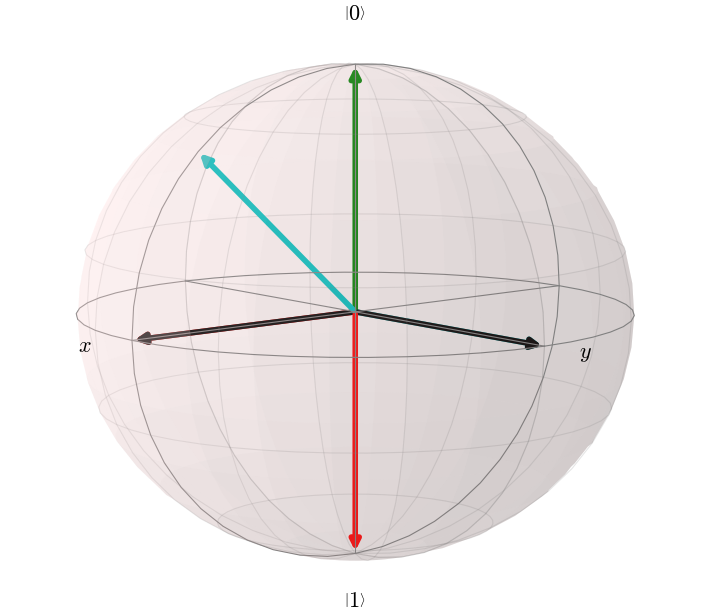
\includegraphics[scale=0.5]{img/bloch3over4.png}
       \caption{Simple binary classification problem of a quantum state}
\end{figure}

\begin{equation}
\frac{1}{\sqrt{2M}}\sum_{m=1}^{M} (\textcolor{emerald}{\ket{0}}\ket{\textcolor{red}{\Psi_{\tilde{x}} (\star)}}+\textcolor{emerald}{\ket{1}}\ket{\textcolor{darkyellow}{\Psi}_{\textcolor{purple}{x^{m}}}})\ket{y^{m}(\textcolor{darkyellow}{A} \ or \ \textcolor{purple}{B})}\ket{m}
\end{equation}
Procedure to load the input vector $\tilde{x}$:
\begin{equation}
\ket{\Psi_0} = \frac{1}{2}\sum_{m=1}^{2} (\textcolor{emerald}{\ket{0}}\ket{0}+\textcolor{emerald}{\ket{1}}\ket{0})\ket{y^{m}}\ket{m}
\end{equation}
Apply controlled rotation $_0^1CR_y(\frac{\pi}{4})$ s.t.
\begin{equation}
_0^1CR_y(\frac{\pi}{4})\ket{\Psi_0} = \ket{\Psi_1} = \frac{1}{2}\sum_{m=1}^{2} (\textcolor{emerald}{\ket{0}}\ket{0}+\textcolor{emerald}{\ket{1}}\ket{\textcolor{red}{\Psi_{\tilde{x}}}})\ket{y^{m}}\ket{m}
\end{equation}
Flip the ancilla qubit in the first register
\begin{equation}
(X\otimes\mathbb{1}\otimes\mathbb{1}\otimes\mathbb{1})\ket{\Psi_1} = \ket{\Psi_2} = \frac{1}{2}\sum_{m=1}^{2} (\textcolor{emerald}{\ket{0}}\ket{\textcolor{red}{\Psi_{\tilde{x}}}}+\textcolor{emerald}{\ket{1}}\ket{0})\ket{y^{m}}\ket{m}
\end{equation}

\subsubsection{Controlled U Gate}
\label{subsubsubsec:controlledugate}

Often there is a need for applying certain quantum gates in a controlled manner. Thus a controlled U (CU) gate is required whereby U can be any unitary single-qubit gate. The CU gate is defined as:

\begin{equation}
CU = \begin{pmatrix}
 \mathbb{1} & 0 \\ 
 0 & U
 \end{pmatrix}
\end{equation}

It is important to note that the CNOT gate is essentially a CU gate in the case of U = X. 

Most of the time the CU gate cannot be implemented directly and has to be realized through larger quantum circuits consisting of CNOT and single-qubit gates. \citeA{nielsen2010quantum} describe such a decomposition as shown in Fig.~\ref{img:cudecomposition}.

\begin{figure}[ht]
   \centering
   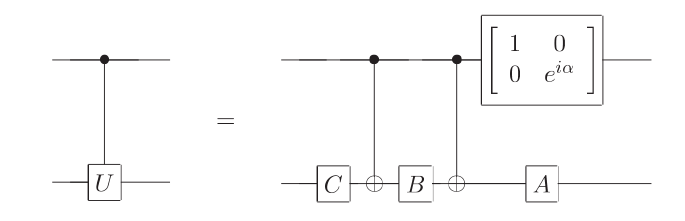
\includegraphics[width=0.7\textwidth]{img/controlledudecomp.png}
   \caption{Circuit decomposition for a controlled-U operation for single-qubit gate U.\textsuperscript{3}}
   \label{img:cudecomposition}
\end{figure}

\footnotetext[3]{Reprinted from Michael A. Nielsen and Isaac L. Chuang. Quantum Computation and Quantum Information. Cambridge University Press, 2000. Copyright 2010 by Nielsen \& Chuang.}

The idea is that when the control qubit is \0 the gate combination ABC is applied to the target qubit and has to equal the identity gate:

\begin{equation}
ABC = \mathbb{1}
\end{equation}

If and only if the control qubit is \1 then the gate sequence $e^{i\alpha}AXBXC$ is applied to the target. Since the goal is to apply the unitary U to the target qubit the following equation must be satified,

\begin{equation}
e^{i\alpha}AXBXC = U
\end{equation}

In order to find the matrices A,B,C and the additional parameter $\alpha$ the following equation has to be solved:

\begin{equation}
U = \begin{pmatrix}
 e^{i(\alpha-\frac{\beta}{2}-\frac{\delta}{2})}\cos{\frac{\gamma}{2}} & -e^{i(\alpha-\frac{\beta}{2}+\frac{\delta}{2})}\sin{\frac{\gamma}{2}} \\ 
e^{i(\alpha+\frac{\beta}{2}-\frac{\delta}{2})}\sin{\frac{\gamma}{2}} & e^{i(\alpha+\frac{\beta}{2}+\frac{\delta}{2})}\cos{\frac{\gamma}{2}}
 \end{pmatrix}
\end{equation}

In our case we need to find A, B, C and $\alpha$ for $_0^1CR_y(\frac{\pi}{4})$:

Using a root finding algorithm for non-linear equations we find:

\begin{equation}
\alpha =  \pi; \quad 
\beta = 2\pi;\quad 
\delta = \frac{7}{8}\pi;\quad 
\gamma = 0
\end{equation}
Then,
\begin{align}
A \quad= \quad R_z(\beta)R_y(\frac{\gamma}{2})\quad =& \quad R_z(2\pi) \quad = \quad \textcolor{emerald}{\mathbb{1}} \\
B\quad =\quad R_y(-\frac{\gamma}{2})R_z(-\frac{\delta+\beta}{2})\quad =& \quad R_z(-\frac{23}{16}\pi) \quad= \quad \textcolor{red}{???}  \\
C \quad=\quad R_z(\frac{\delta-\beta}{2})\quad =& \quad R_z(-\frac{9}{16}\pi) \quad= \quad \textcolor{red}{???} \\
\begin{pmatrix} 1&0\cr0&e^{i\alpha} \end{pmatrix}\quad=& \quad \begin{pmatrix} 1&0\cr0&e^{i\pi} \end{pmatrix}\quad= \quad \textcolor{emerald}{Z}
\end{align}


The Solovay-Kitaev theorem

\begin{align}
B\quad =&\quad R_z(-\frac{23}{16}\pi) \quad= \quad \textcolor{red}{???}  \\
C \quad=&\quad R_z(-\frac{9}{16}\pi) \quad= \quad \textcolor{red}{???}
\end{align}

The Solovay-Kitaev theorem guarantees that given a set of single-qubit quantum gates which generates a dense subset of $SU(2)$, then that set is guaranteed to fill $SU(2)$ quickly.\cite{dawson2005solovay}.
 
$\rightarrow$ \textcolor{emerald}{\textbf{Hence, given any universal gate set it is possible to obtain good approximations to any desired gate.}}

$\rightarrow$ \textcolor{red}{\textbf{But needs to be computed classically!}}

\begin{redbox}
Fowler distance\textsuperscript{1}:
\begin{equation}
dist(U,U_{approx}) = \sqrt{\frac{2-\mid tr(U\cdot U_{approx}^\dagger)\mid}{2}}
\end{equation}
\cite{booth2012quantum}
\end{redbox}

\begin{figure}
\centering
    \begin{tikzpicture}[scale=0.8]
\begin{axis}[xlabel={Gate count},ylabel={Fowler distance [$d(U,U_{approx})$]}]

% Graph column 2 versus column 0
\addplot table[x index=1,y index=0,col sep=comma] {datax.dat};
\addlegendentry{$R_z(-\frac{9}{16}\pi)$}% y index+1 since humans count from 1

% Graph column 1 versus column 0    
\addplot table[x index=5,y index=4,col sep=comma] {datax.dat};
\addlegendentry{$R_z(-\frac{23}{16}\pi)$}

\end{axis}
\end{tikzpicture}
  \end{figure}

\begin{minipage}[c]{.8\textwidth}
	%\vspace{-20mm}
	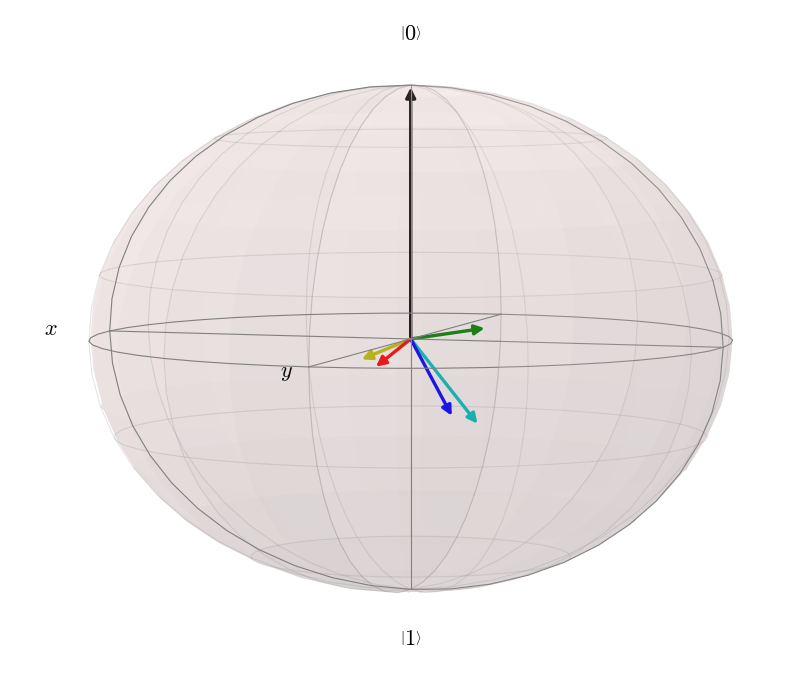
\includegraphics[height=0.8\textwidth]{img/fowlerdistance.png}
       \captionsetup{justification=raggedright, singlelinecheck=false}
       \captionof{figure}{Various Fowler distances visualized on Bloch sphere }
\end{minipage}%%%%%
\begin{minipage}[c]{.2\textwidth}
\scriptsize
\begin{equation}
\textcolor{cyan}{d = 0.22739}
\end{equation}
\begin{equation}
\textcolor{emerald}{d = 0.15165}
\end{equation}
\begin{equation}
\textcolor{blue}{d = 0.10722}
\end{equation}
\begin{equation}
\textcolor{darkyellow}{d = 0.02086}
\end{equation}
\begin{equation}
\textcolor{red}{d = 0.00156}
\end{equation}

\end{minipage}

\begin{table}
\centering
    \begin{tabular}{c| c |c |c }
      \toprule
      Approx. Gate & Fowler distance & Gate count & Execution time\\
      \midrule
      $R_z(-\frac{23}{16}\pi)$ & 0.15165 & 25 & \textcolor{emerald}{$\sim$\SI{3}{\micro\second}}\\
       & 0.10722 & 109 & \textcolor{emerald}{$\sim$\SI{14}{\micro\second}}\\
       & 0.02086 & 2997 & \textcolor{red}{$\sim$\SI{390}{\micro\second}}\\
       & 0.01494 & 14721 & \textcolor{red}{$\sim$\SI{1914}{\micro\second}}\\
       & 0.003327 & 74009 & \textcolor{red}{$\sim$\SI{9621}{\micro\second}}\\
       & 0.001578 & 370813 & \textcolor{red}{$\sim$\SI{48206}{\micro\second}}\\
      \bottomrule
    \end{tabular}
    \caption{SK algorithm results}
  \end{table}

Adding complexities

Executing the SK algorithm adds to our overall algorithmic complexity:

\begin{greenbox}
Overall algorithmic complexity

	$\mathcal{O}(\frac{1}{p_{acc}})+\mathcal{O}(k)+\textcolor{red}{\mathcal{O}(m*log^{2.71}(\frac{m}{\epsilon}))}$ for $\epsilon$-approximations of $m$ gates
	
Cite \cite{dawson2005solovay}
	
Due to state preparation we went from
\begin{equation}  
\mathcal{O}(\frac{1}{p_{acc}})
\end{equation}
suddenly to 
\begin{equation}
\mathcal{O}(m*log^{2.71}(\frac{m}{\epsilon}))
\end{equation}
where $m$ is the number of gates that need approximation to $\epsilon$-accuracy
\end{greenbox}

\newpage

STEPPING UP THE GAME SINCE IBM DOESN'T WORK SO FAR
\subsection{Simulating the amplitude-based kNN algorithm}
\label{subsubsec:simulationamplitudeKNN}

\subsubsection{Diffusion matrix from quantum random walks}
\label{subsubsubsec:diffusion}

Initialization of amplitude distribution is non-trivial

Need for a simpler way - using diffusion matrix from quantum random walks

For the simplest case, consider the entries in the classical probability vector v to be normal distributed, e.g.

CHECK THE ORDER!
\begin{equation}
v = \colvec{0.064180\\0.146860\\0.146770\\0.341590\\0.026840\\0.063590\\0.061700\\0.148470}
\end{equation}

The goal is to encode this classical data into a quantum memory state $\ket{M}$ of the form,

\begin{align}
\ket{M} = \quad &0.064180 \ket{000} +
0.146860 \ket{100} +
0.146770 \ket{010} +
0.341590 \ket{001}\notag\\
&+ 0.026840 \ket{110}
+ 0.063590 \ket{011} +
0.061700 \ket{101} +
0.148470 \ket{111}
\end{align}

%Before outlining how to prepare state $\ket{M}$ the notion of Hamming distance needs to be introduced.

Furthermore, a useful tool of visualizing the HDs between binary patterns made from three qubits is a 3-D cube as shown in Fig.~\ref{img:cubenoprobs}. On the cube, adjacent qubit patterns have a HD of 1 and the HD increases by 1 for every additional corner. For example, the qubit state $\ket{000}$ is adjacent to $\ket{100}$ since they only differ in one qubit ($HD=1$). Moving one more corner yields the state $\ket{101}$ or $\ket{110}$ which both have a HD of 2 compared to $\ket{000}$.

\begin{figure}[!ht]
       \centering
       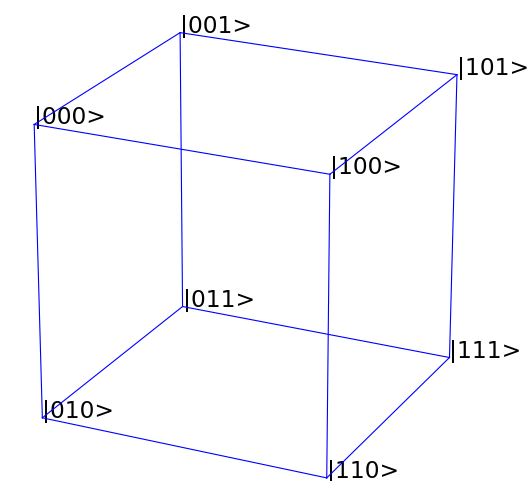
\includegraphics[width=0.5\textwidth]{img/cubewithoutprobs.png}
       \caption{\label{img:cubenoprobs} Visualizing Hamming distances on a 3-D cube}
\end{figure}

This way of visualizing HDs can be extended to the 16 binary patterns made by four qubits that can be visualized on a 4-D cube, also called tesseract, as illustrated in Fig.~\ref{img:hypercubenoprobs}.

\begin{figure}[!ht]
       \centering
       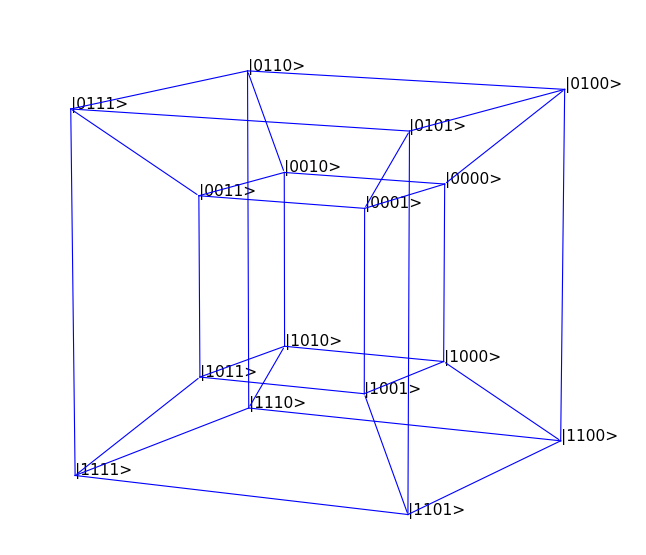
\includegraphics[width=0.5\textwidth]{img/hypercubewithoutprobs.png}
       \caption{\label{img:hypercubenoprobs} Visualizing Hamming distances on a 4-D cube (tesseract)}
\end{figure}

The idea of a coin operator $C$ can be borrowed from the theory of quantum random walks to initialize a gaussian distribution centered around a chosen binary qubit pattern. For this purpose, the coin operator is defined as,

\begin{equation}
C = \begin{pmatrix}
\sqrt{\delta} & 1-\sqrt{\delta} \\
1-\sqrt{\delta} & -\sqrt{\delta}
\end{pmatrix}
\end{equation}

where $0 \leq \delta \leq 1$.